\documentclass[9pt,twocolumn,twoside]{styles/osajnl}
\usepackage{fancyvrb}
\journal{i524} 

\title{Prototyping a Virtual Robot Swarm with ROS and Gazebo}

\author[1]{Matthew Lawson}
\author[1,*]{Gregor von Laszewski}

\affil[1]{School of Informatics and Computing, Bloomington, IN 47408, U.S.A.}

\affil[*]{Corresponding authors: laszewski@gmail.com}

\dates{project-000, \today}

\ociscodes{Cloud, I524, ROS, Gazebo, Robot, Swarm}

% replace this with your url in github/gitlab
\doi{\url{https://github.com/cloudmesh/classes/blob/master/docs/source/format/report/report.pdf}}


\begin{abstract}
Our virtual robot swarm prototype accomplishes a \textit{TBD task} by allocating portions of the task to each virtual robot (VR).  As each VR works on its piece of the task, it communicates relevant information back to the master VR.  Upon completion, the master VR collates the results and creates a human-readable report.  The virtual swarm utilizes the \textit{Robot Operating System} to control the virtual robots, \textit{Gazebo} to simulate the task completion and \textit{RVIZ} to visualize the process.  We use \textit{Ansible} to deploy the software to a distributed computing environment.  Th importance of our effort centers on some super-special conclusion I do not yet grasp.
\newline
\end{abstract}

\setboolean{displaycopyright}{true}

\begin{document}

\maketitle

\section{Introduction}
Stating the Problem:
Simulating a single robot's actions and responses to its environment prior to real-world deployment mitigates risk and improves results at a relatively low cost. It follows that simulating the actions and responses of a group of robots, e.g., a swarm, will also improve results at a low cost.  However, deployment of an interconnected swarm of virtual robots requires much more time and effort than a single virtual robot.  Collecting the results from a swarm also requires additional effort.

Our Contribution:
We create a cross-platform system to quickly and relatively easily deploy and manage a swarm, as well as evaluate the swarm's operational effectiveness.  Or maybe something else...I'm not sure, yet.
Automate the deployment of a virtual robot swarm that will accomplish some arbitrary task; capture data from the swarm as it completes its task; report back the results in a human-readable format.

\section{Virtual Robot Swarm Components}
\subsection{Robot Operating System (ROS)}
TBD; will include a discussion of a) how to obtain and install ROS and b) ROS graph concepts.  The latter topic will introduce ROS' core components, namely a node, publications, suscriptions, topics and services.  This section should probably cover ROS packages and ROS client libraries (primarily C++ and Python)
\subsection{Gazebo}
TBD; again, introducing core Gazebo concepts.  In this case, will include a) world files, b) model files and c) its client-server model.  It should also include non-obvious limitation examples, e.g., a gripper arm driven by a single screw instead of multiple screws.  In addition, it should allude to any limitations that affect our simulation.
\subsection{Ansible}
TBD; briefly describe Ansible - what it is, salient features, etc.
\subsection{Testing Environment}
TBD; briefly describe cloudmesh


\section{Virtual Robot Swarm Project Implementation}
\subsection{VR Swarm task}
TBD; discuss the task to be accomplished by the swarm, as well as how the information collected during task completion will be communicated back to the master node for collation and reporting.
\subsection{Deployment}
TBD; document the Ansible steps needed to successfully deploy ROS and Gazebo on multiple computers;  will include references for obtaining major components, including adding new repositories if needed.
\subsection{Modifications, Pitfalls}
TBD; discuss any obstacles encountered with deployment due to dependency problems, connecting ROS and Gazebo, etc.
\subsection{Initializing the Swarm}
TBD; starting ROS and Gazebo to create the virtual environment; testing swarm interconnectivity; designating master node, etc.
\subsection{Begin Task and Monitor Swarm's Progress}
TBD; discuss the steps to initiate task completion and monitor the swarm's progress;
\subsection{Information Acquired}
TBD; discuss the iformation obtained from the swarm wrt the task at hand as well as each node's vital signs, e.g., battery level;
\subsection{Updating Software}
TBD; discuss the methods used to implement software updates on each node; remain cognizant of battery levels
\textit{I have no idea how I might accomplish an over-the-air update of ROS.  This point intimidates me.}

\section{VR Swarm Project Conclusions}
TBD; present the data collected in some visualization format; discuss why this project advances robotics forward by utilizing distributed computing;

\section{Examples of Article Components}
\label{sec:examples}

The sections below show examples of different article components.

\section{Figures and Tables}

It is not necessary to place figures and tables at the back of the
manuscript. Figures and tables should be sized as they are to appear
in the final article. Do not include a separate list of figure
captions and table titles.

Figures and Tables should be labelled and referenced in the standard
way using the \verb|\label{}| and \verb|\ref{}| commands.

\subsection{Sample Figure}

Figure \ref{fig:false-color} shows an example figure.

\begin{figure}[htbp]
\centering
\fbox{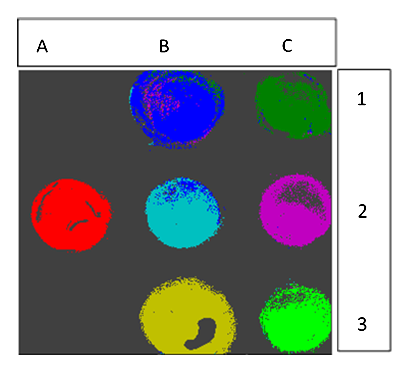
\includegraphics[width=\linewidth]{images/sample}}
\caption{False-color image, where each pixel is assigned to one of seven reference spectra.}
\label{fig:false-color}
\end{figure}

\subsection{Sample Table}

Table \ref{tab:shape-functions} shows an example table.

\begin{table}[htbp]
\centering
\caption{\bf Shape Functions for Quadratic Line Elements}
\begin{tabular}{ccc}
\hline
local node & $\{N\}_m$ & $\{\Phi_i\}_m$ $(i=x,y,z)$ \\
\hline
$m = 1$ & $L_1(2L_1-1)$ & $\Phi_{i1}$ \\
$m = 2$ & $L_2(2L_2-1)$ & $\Phi_{i2}$ \\
$m = 3$ & $L_3=4L_1L_2$ & $\Phi_{i3}$ \\
\hline
\end{tabular}
  \label{tab:shape-functions}
\end{table}

\section{Sample Equation}

Let $X_1, X_2, \ldots, X_n$ be a sequence of independent and
identically distributed random variables with $\text{E}[X_i] = \mu$
and $\text{Var}[X_i] = \sigma^2 < \infty$, and let

\begin{equation}
S_n = \frac{X_1 + X_2 + \cdots + X_n}{n}
      = \frac{1}{n}\sum_{i}^{n} X_i
\label{eq:refname1}
\end{equation}

denote their mean. Then as $n$ approaches infinity, the random
variables $\sqrt{n}(S_n - \mu)$ converge in distribution to a normal
$\mathcal{N}(0, \sigma^2)$. 

\section{Sample Algorithm}

Algorithms can be included using the commands as shown in algorithm
\ref{alg:euclid}.

\begin{algorithm}
\caption{Euclid’s algorithm}\label{alg:euclid}
\begin{algorithmic}[1]
\Procedure{Euclid}{$a,b$}\Comment{The g.c.d. of a and b}
\State $r\gets a\bmod b$
\While{$r\not=0$}\Comment{We have the answer if r is 0}
\State $a\gets b$
\State $b\gets r$
\State $r\gets a\bmod b$
\EndWhile\label{euclidendwhile}
\State \textbf{return} $b$\Comment{The gcd is b}
\EndProcedure
\end{algorithmic}
\end{algorithm}

\begin{algorithm}
\caption{Python example}\label{alg:python}
\begin{quote}
\begin{Verbatim}[numbers=left]
for i in range(0,100):
  print i
\end{Verbatim}
\end{quote}
\end{algorithm}

\section{Reference Management}

The best programs to manage your references is jabref or emacs. You
can edit the references and verify them with them for format
errors. To cite them use the citation key. You can add multiple bib
files to the bibliography command separated by comma.

\noindent Add citations with the cite command. See
\cite{las14cloudmeshmultiple} for an example on how to use multiple
clouds. In \cite{www-i524} we list the class content.

Here a test of a citation with an underscore in the url \cite{www-underscore}.

\section{Supplemental Material}

% Bibliography

\bibliography{references}
 
\section*{Author Biographies}
\begingroup
\setlength\intextsep{0pt}
\begin{minipage}[t][3.2cm][t]{1.0\columnwidth} % Adjust height [3.2cm] as required for separation of bio photos.
  \begin{wrapfigure}{L}{0.25\columnwidth}
    
\includegraphics[width=0.25\columnwidth]{images/john_smith.eps}
  \end{wrapfigure}
  \noindent
  {\bfseries John Smith} received his BSc (Mathematics) in 2000 from
  The University of Maryland. His research interests include lasers
  and optics. 
\end{minipage}
\begin{minipage}[t][3.2cm][t]{1.0\columnwidth} % Adjust height [3.2cm] as required for separation of bio photos.
  \begin{wrapfigure}{L}{0.25\columnwidth}
    
\includegraphics[width=0.25\columnwidth]{images/alice_smith.eps}
  \end{wrapfigure}
  \noindent
  {\bfseries Alice Smith} received her BSc (Mathematics) in 2000 from
  The University of Maryland. Her research interests also include
  lasers and optics. 
\end{minipage}
\begin{minipage}[t][3.2cm][t]{1.0\columnwidth} % Adjust height [3.2cm] as required for separation of bio photos.
  \begin{wrapfigure}{L}{0.25\columnwidth}
    
\includegraphics[width=0.25\columnwidth]{images/alice_smith.eps}
  \end{wrapfigure}
  \noindent
  {\bfseries Bruce Wayne} received his BSc (Aeronautics) in 2000 from
  Indiana University. His research interests include lasers and optics.
\end{minipage}
\endgroup

\newpage

\appendix

\section{Work Breakdown}

The work on this project was distributed as follows between the
authors:

\begin{description}

\item[Matthew Lawson.] Designed the project in collaboration w/ Gregor von Laszewski, researched the material and implemented the project.  Slept far too little.

\item[Gregor von Laszewski.] Provided invaluable insights at key points during the process.

\end{description}

\section{Report Checklist}

\begin{itemize}
\renewcommand{\labelitemi}{\scriptsize$\square$} 
\item Have you written the report in word or LaTeX in the specified
  format?
\item Have you included the report in github/lab?
\item Have you specified the names and e-mails of all team members in
  your report. E.g. the username in Canvas?
\item Have you included the HID of all team members?
\item Does the report have the project number added to it?
\item Have you included all images in native and PDF format in gitlab
  in the images folder?
\item Have you added the bibliography file in bibtex format?
\item Have you submitted an additional page that describes who did
  what in the project or report?
\item Have you spellchecked the paper?
\item Have you made sure you do not plagiarize?
\item Have you made sure that the important directories are all lower
  case and have no underscore or space in it?
\item Have you made sure that all authors have a README.rst in their
  HID github/lab repository?
\item Have you made sure that there is a README.rst in the project
  directory and that it is properly filled out?
\item Have you put a work breakdown in the document if you worked in a
  group?
\end{itemize}
\end{document}